\documentclass[unknownkeysallowed]{beamer}
\usepackage[french,english]{babel}
\usepackage{../sty/beamer_js}
\usepackage{../sty/shortcuts_js}

\usepackage{dirtree}
\newcommand{\Benchopt}{\texttt{Benchopt}}

\definecolor{tomcolor}{rgb}{0.,.3,.6}
\lstset{basicstyle=\color{tomcolor}\scriptsize\ttfamily}
\addbibresource{../biblio/biblio.bib}
\captionsetup[subfigure]{labelformat=empty}
\begin{document}

%%%%%%%%%%%%%%%%%%%%%%%%%%%%%%%%%%%%%%%%%%%%%%%%%%%%%%%%%%%%%%%%%%%%%%%%%%%%%%%
%%%%%%%%%%%%%%%%%%%%%%             Headers               %%%%%%%%%%%%%%%%%%%%%%
%%%%%%%%%%%%%%%%%%%%%%%%%%%%%%%%%%%%%%%%%%%%%%%%%%%%%%%%%%%%%%%%%%%%%%%%%%%%%%%


%%%%%%%%%%%%%%%%%%%%%%%%%%%%%%%%%%%%%%%%%%%%%%%%%%%%%%%%%%%%%%%%%%%%%%%%%%%%%%%
\begin{frame}
\bigskip
\bigskip
\begin{center}{
\LARGE\color{marron}
\textbf{\texttt{Benchopt}:\\
Reproducible, efficient and collaborative optimization benchmarks}
\textbf{ }\\
}

\color{marron}
\end{center}

\vspace{0.5cm}

\begin{center}
\textbf{Benchopt contributors} \\
\vspace{0.1cm}
\url{https://benchopt.github.io}\\
\end{center}

\centering

\includegraphics[width=0.43\textwidth]{../sharedimages/benchopt_logo.pdf}

\end{frame}
%%%%%%%%%%%%%%%%%%%%%%%%%%%%%%%%%%%%%%%%%%%%%%%%%%%%%%%%%%%%%%%%%%%%%%%%%%%%%%%

%%%%%%%%%%%%%%%%%%%%%%%%%%%%%%%%%%%%%%%%%%%%%%%%%%%%%%%%%%%%%%%%%%%%%%%%%%%%%%%
\begin{frame}{Contributors from...}
    \centering
    
\includegraphics[width=100px]{../sharedimages/logo_inria_horiz.pdf} \hspace{1mm}
    \includegraphics[height=45px]{../sharedimages/um_logo.pdf} \hspace{1mm}
    
\includegraphics[height=35px]{../sharedimages/logo_berkeley.png} \hspace{1mm}
    \\[7mm]
    
\includegraphics[height=50px]{../sharedimages/logo_cnrs.pdf} \hspace{5mm}
    
\includegraphics[height=50px]{../sharedimages/logo_lund} \hspace{5mm}
    
\includegraphics[height=50px]{../sharedimages/logo_telecom.pdf} \hspace{5mm}
    
\includegraphics[height=50px]{../sharedimages/logo_univ_luxembourg.pdf} \\[4mm]
    
\includegraphics[height=40px]{../sharedimages/logo_ens.png}
    % \includegraphics[height=40px]{../sharedimages/}
\end{frame}
%%%%%%%%%%%%%%%%%%%%%%%%%%%%%%%%%%%%%%%%%%%%%%%%%%%%%%%%%%%%%%%%%%%%%%%%%%%%%%%



%%%%%%%%%%%%%%%%%%%%%%%%%%%%%%%%%%%%%%%%%%%%%%%%%%%%%%%%%%%%%%%%%%%%%%%%%%%%%%%
\begin{frame}{Benchmarking algorithms is a pain}

Machine Learning research relies on numerical validation.

\vskip2em

Pain points of a benchmark:\\[.2em]
\begin{itemize}
	\item competitors' methods do not work out of the box.
	\item re-code methods and tools to integrate a new method.
	\item hard to extend with new settings.
\end{itemize}
\vskip1em
{\centering \large all of this started from scratch by every submission!\\}
% \end{minipage}

\vskip2em


\Benchopt{} produces \textbf{open}, \textbf{reproducible}, \textbf{extendable} benchmarks

\end{frame}
%%%%%%%%%%%%%%%%%%%%%%%%%%%%%%%%%%%%%%%%%%%%%%%%%%%%%%%%%%%%%%%%%%%%%%%%%%%%%%%



%%%%%%%%%%%%%%%%%%%%%%%%%%%%%%%%%%%%%%%%%%%%%%%%%%%%%%%%%%%%%%%%%%%%%%%%%%%%%%%
\begin{frame}{How does \Benchopt{} do it?}

\Benchopt{} is a framework to organize and run benchmarks:
\begin{itemize}
    \item one repository per benchmark
    \item one base open source \texttt{Python} CLI to run them
\end{itemize}

\vskip1em
Examples of existing benchmarks:
\vskip.5em
\begin{minipage}{0.45\linewidth}
    {\small
    \begin{itemize}
        \item Resnet18
        \item Lasso
        \item ICA
        \item Logistic regression
    \end{itemize}
    }
\end{minipage}
\begin{minipage}{0.48\linewidth}
    {\small
    \begin{itemize}
        \item Total Variation
        \item Ordinary Least Squares
        \item Non convex sparse regression
        \item linear SVM
    \end{itemize}
    }
\end{minipage}
\vskip2em

\centering
Start yours with \url{https://github.com/benchopt/template_benchmark}!
\end{frame}
%%%%%%%%%%%%%%%%%%%%%%%%%%%%%%%%%%%%%%%%%%%%%%%%%%%%%%%%%%%%%%%%%%%%%%%%%%%%%%%


%%%%%%%%%%%%%%%%%%%%%%%%%%%%%%%%%%%%%%%%%%%%%%%%%%%%%%%%%%%%%%%%%%%%%%%%%%%%%%%
\begin{frame}{Components of a benchmark}

    \centering
    \vspace*{-5mm}
    \textbf{3 components}: Objective, Dataset, Solver

    \vskip3em
    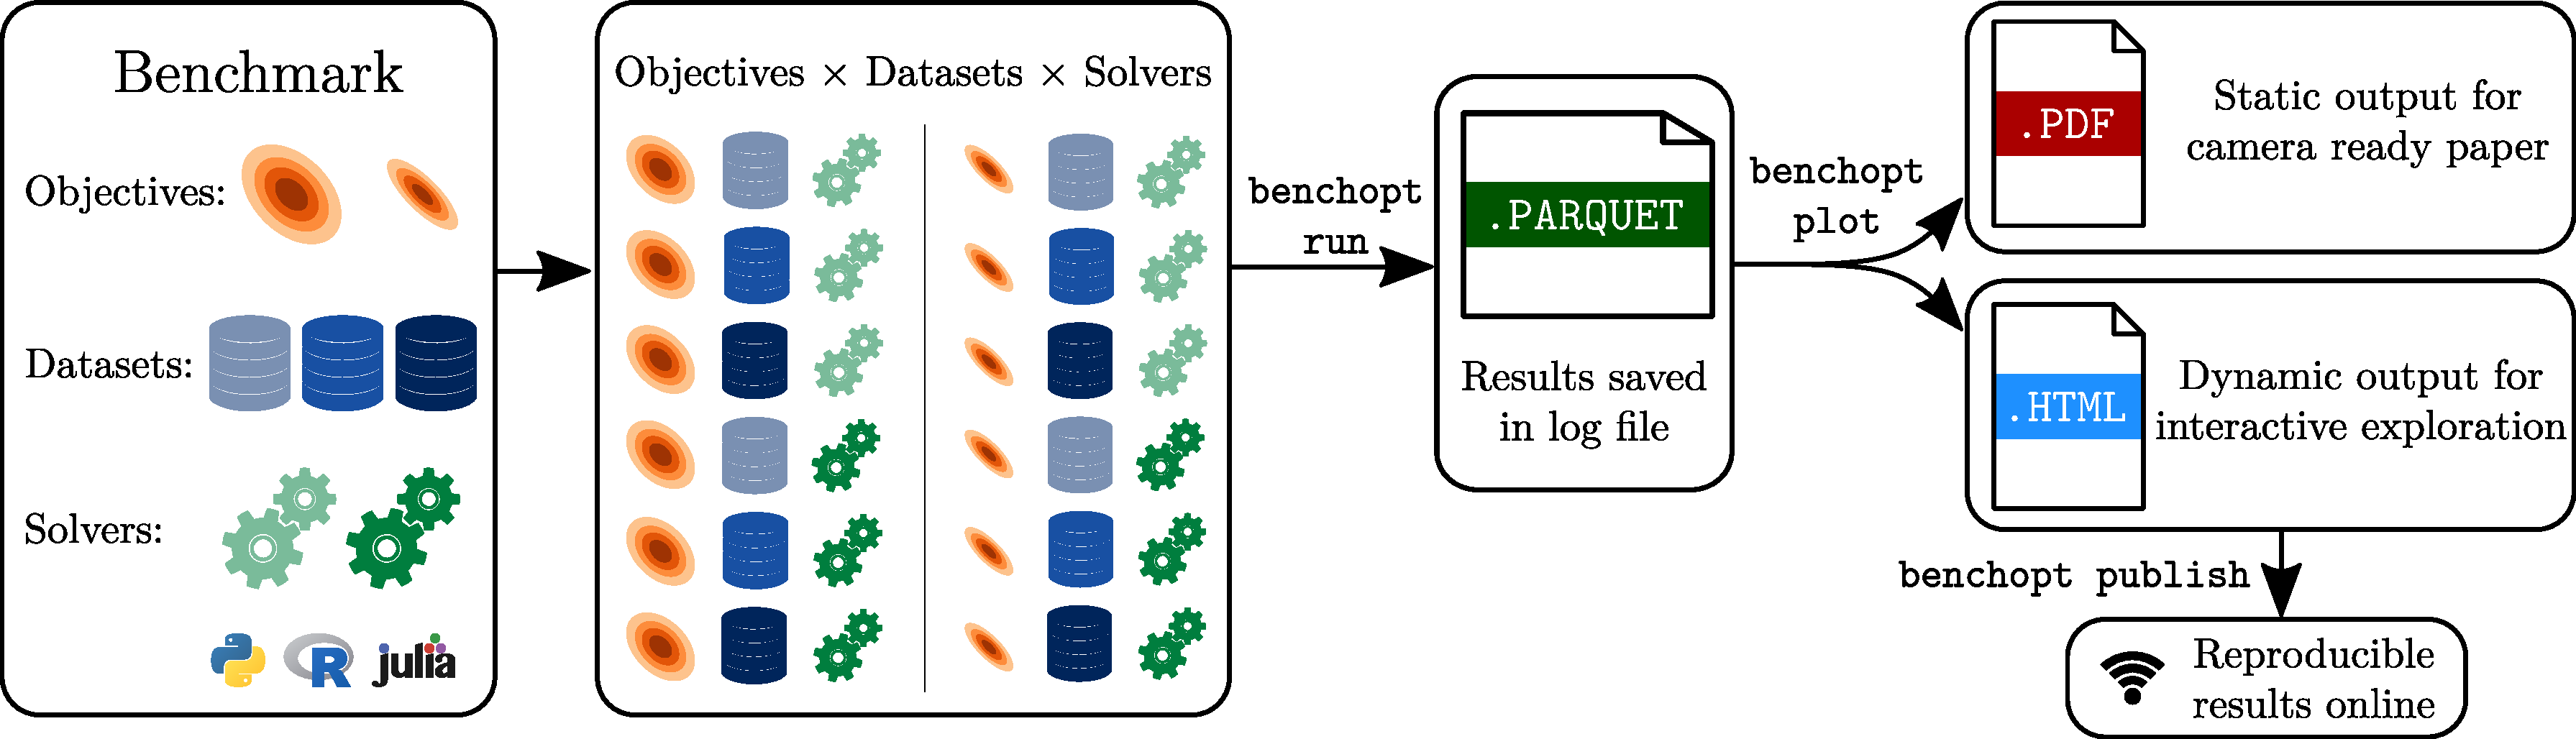
\includegraphics[width=\linewidth]{../sharedimages/benchopt_schema.pdf}

\end{frame}
%%%%%%%%%%%%%%%%%%%%%%%%%%%%%%%%%%%%%%%%%%%%%%%%%%%%%%%%%%%%%%%%%%%%%%%%%%%%%%%



%%%%%%%%%%%%%%%%%%%%%%%%%%%%%%%%%%%%%%%%%%%%%%%%%%%%%%%%%%%%%%%%%%%%%%%%%%%%%%%
\begin{frame}{Structure of a benchmark}

    \begin{minipage}{0.45\linewidth}
        \dirtree{%
        .1 benchmark/.
        .2 objective.py.
        .2 datasets/.
        .3 dataset1.py.
        .3 dataset2.py.
        .2 solvers/.
        .3 solver1.py.
        .3 solver2.py.
    }
    \end{minipage}
    \begin{minipage}{0.45\linewidth}

    \textbf{Modular \& extendable}
    \vspace*{5mm}

    New solver? add a file

    New dataset? add a file

    New metric? modify objective
    \end{minipage}

\end{frame}
%%%%%%%%%%%%%%%%%%%%%%%%%%%%%%%%%%%%%%%%%%%%%%%%%%%%%%%%%%%%%%%%%%%%%%%%%%%%%%%

%%%%%%%%%%%%%%%%%%%%%%%%%%%%%%%%%%%%%%%%%%%%%%%%%%%%%%%%%%%%%%%%%%%%%%%%%%%%%%%
\begin{frame}{Interactive results exploration}
    \centering
    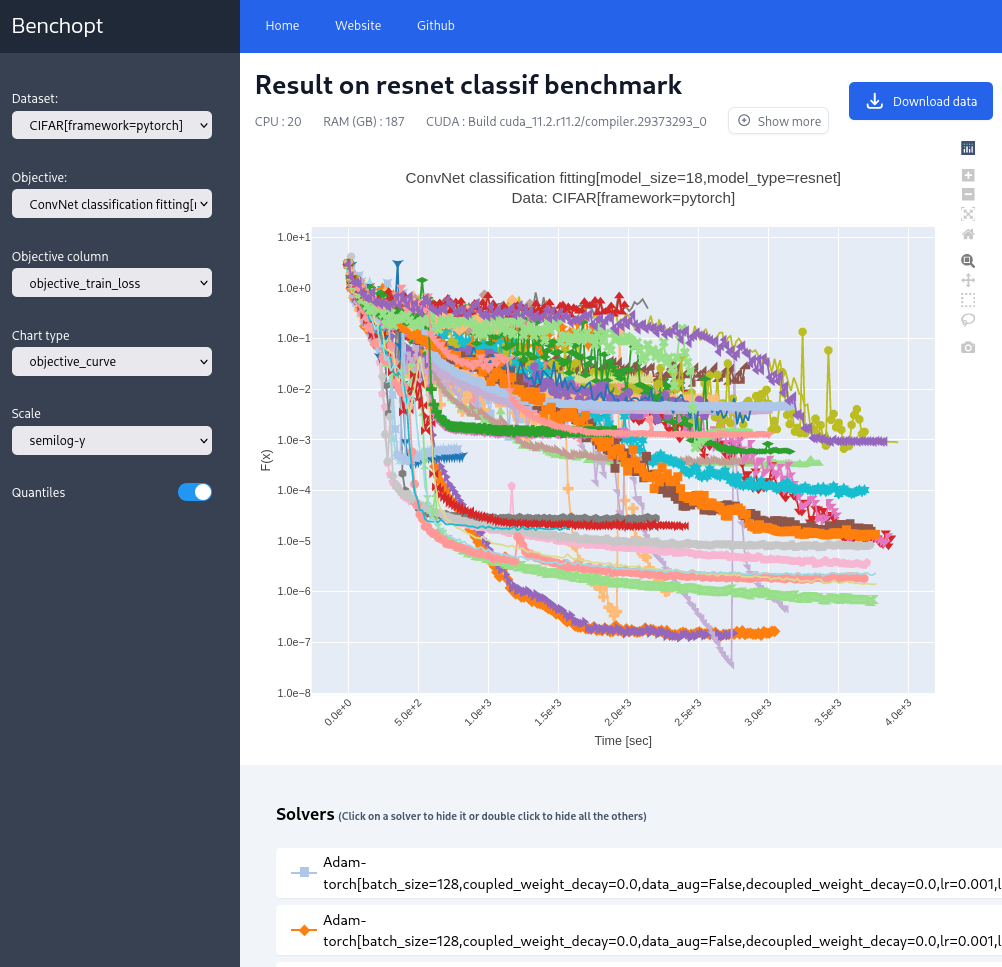
\includegraphics[width=0.8\linewidth]{../sharedimages/benchopt_convnet.png}
\end{frame}
%%%%%%%%%%%%%%%%%%%%%%%%%%%%%%%%%%%%%%%%%%%%%%%%%%%%%%%%%%%%%%%%%%%%%%%%%%%%%%%


%%%%%%%%%%%%%%%%%%%%%%%%%%%%%%%%%%%%%%%%%%%%%%%%%%%%%%%%%%%%%%%%%%%%%%%%%%%%%%%
\begin{frame}{\Benchopt{} makes your life easy}

    \begin{itemize}
        \item build on previous benchmarks
        \item use solvers in Python, R, Julia, binaries...
        \item monitor any metric you want altogether (test/train loss, ...)
        \item add parameters to solvers
        \item share and publish HTML results
        \item run all benchmarks in parallel
        \item cache results
        \item and much more!
    \end{itemize}
    \vskip1em
    \centering
    
\includegraphics[width=0.8\linewidth]{../sharedimages/tweet_rahimi.png}
\end{frame}
%%%%%%%%%%%%%%%%%%%%%%%%%%%%%%%%%%%%%%%%%%%%%%%%%%%%%%%%%%%%%%%%%%%%%%%%%%%%%%%


%%%%%%%%%%%%%%%%%%%%%%%%%%%%%%%%%%%%%%%%%%%%%%%%%%%%%%%%%%%%%%%%%%%%%%%%%%%%%%%
\begin{frame}{Example: Resnet benchmark}

    { \small
    \begin{itemize}
        \item image classification with resnet18
        \item various optimization strategies
        \item compare \texttt{pytorch} and \texttt{tensorflow}
        \item publish reproducible SOTA for baselines
    \end{itemize}
    }

    \vskip1em
    \centering
    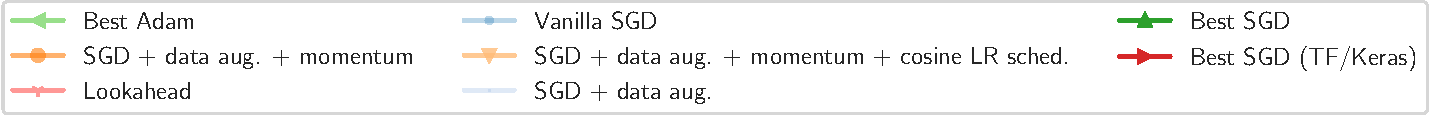
\includegraphics[width=\linewidth]{../sharedimages/resnet18_sgd_torch_legend.pdf}
    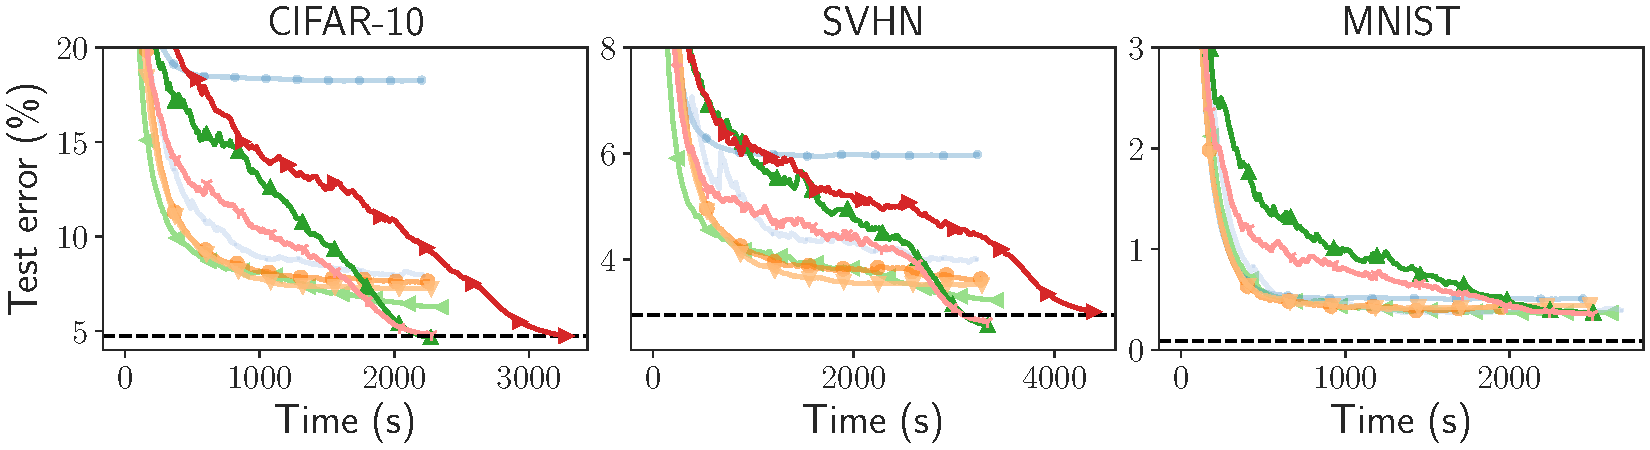
\includegraphics[width=\linewidth]{../sharedimages/resnet18_sgd_torch.pdf}

    \url{https://github.com/benchopt/benchmark_resnet_classif/}
\end{frame}
%%%%%%%%%%%%%%%%%%%%%%%%%%%%%%%%%%%%%%%%%%%%%%%%%%%%%%%%%%%%%%%%%%%%%%%%%%%%%%%




% %%%%%%%%%%%%%%%%%%%%%%%%%%%%%%%%%%%%%%%%%%%%%%%%%%%%%%%%%%%%%%%%%%%%%%%%%%%%%%%
% \begin{frame}{\texttt{benchopt}}
%     \centering
%     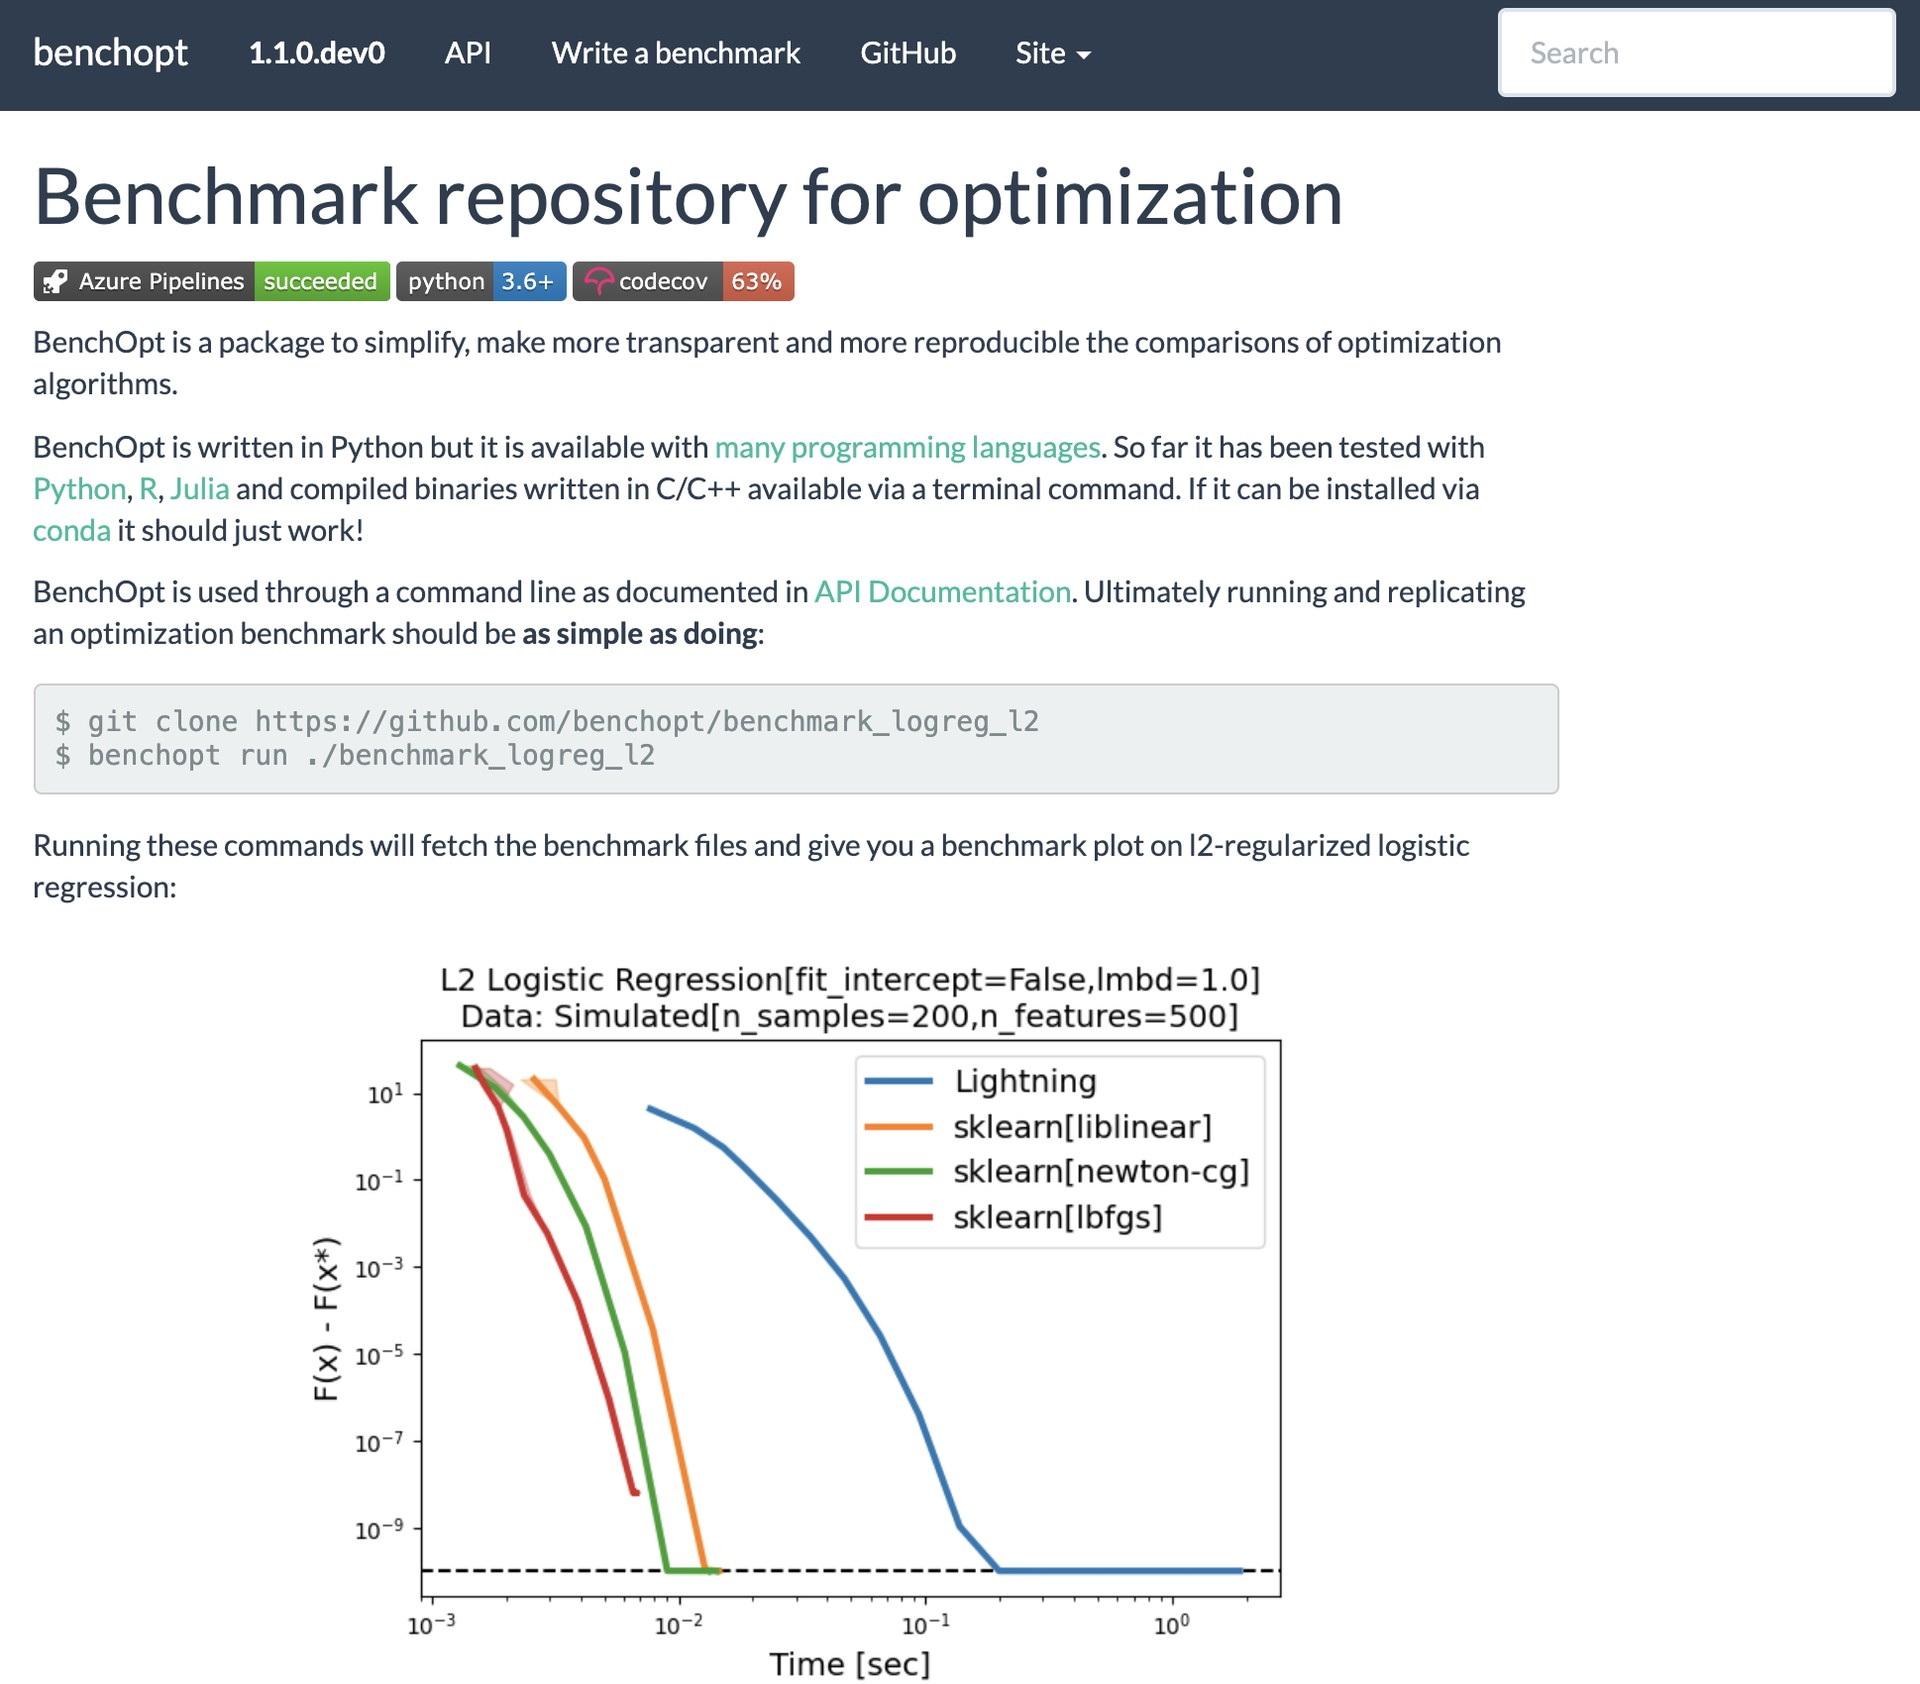
\includegraphics[width=.9\textwidth]{benchopt}\\
% \end{frame}
% %%%%%%%%%%%%%%%%%%%%%%%%%%%%%%%%%%%%%%%%%%%%%%%%%%%%%%%%%%%%%%%%%%%%%%%%%%%%%%%


% %%%%%%%%%%%%%%%%%%%%%%%%%%%%%%%%%%%%%%%%%%%%%%%%%%%%%%%%%%%%%%%%%%%%%%%%%%%%%%%
% \begin{frame}{Contact}

% \vspace{0.4cm}
% \centering
% \includegraphics[width=0.93\textwidth]{contact_js}
% \end{frame}
% %%%%%%%%%%%%%%%%%%%%%%%%%%%%%%%%%%%%%%%%%%%%%%%%%%%%%%%%%%%%%%%%%%%%%%%%%%%%%%%



% %%%%%%%%%%%%%%%%%%%%%%%%%%%%%%%%%%%%%%%%%%%%%%%%%%%%%%%%%%%%%%%%%%%%%%%%%%%%%%%
% % Uncomment for references
% \begin{frame}{Bibliographie}
% \printbibliography
% \end{frame}
%  %%%%%%%%%%%%%%%%%%%%%%%%%%%%%%%%%%%%%%%%%%%%%%%%%%%%%%%%%%%%%%%%%%%%%%%%%%%%%%



\end{document}
